\documentclass[a4paper, 14pt]{extarticle}

% Поля
%--------------------------------------
\usepackage{geometry}
\geometry{a4paper,tmargin=2cm,bmargin=2cm,lmargin=3cm,rmargin=1cm}
%--------------------------------------


%Russian-specific packages
%--------------------------------------
\usepackage[T2A]{fontenc}
\usepackage[utf8]{inputenc} 
\usepackage[english, main=russian]{babel}
%--------------------------------------

\usepackage{textcomp}

% Красная строка
%--------------------------------------
\usepackage{indentfirst}               
%--------------------------------------             


%Graphics
%--------------------------------------
\usepackage{graphicx}
\graphicspath{ {./images/} }
\usepackage{wrapfig}
%--------------------------------------

% Полуторный интервал
%--------------------------------------
\linespread{1.3}                    
%--------------------------------------

%Выравнивание и переносы
%--------------------------------------
% Избавляемся от переполнений
\sloppy
% Запрещаем разрыв страницы после первой строки абзаца
\clubpenalty=10000
% Запрещаем разрыв страницы после последней строки абзаца
\widowpenalty=10000
%--------------------------------------

%Списки
\usepackage{enumitem}

%Подписи
\usepackage{caption} 

%Гиперссылки
\usepackage{hyperref}

\hypersetup {
	unicode=true
}

%Рисунки
%--------------------------------------
\DeclareCaptionLabelSeparator*{emdash}{~--- }
\captionsetup[figure]{labelsep=emdash,font=onehalfspacing,position=bottom}
%--------------------------------------

\usepackage{tempora}

%Листинги
%--------------------------------------
\usepackage{listings}
\lstset{
  basicstyle=\ttfamily\footnotesize, 
  %basicstyle=\footnotesize\AnkaCoder,        % the size of the fonts that are used for the code
  breakatwhitespace=false,         % sets if automatic breaks shoulbd only happen at whitespace
  breaklines=true,                 % sets automatic line breaking
  captionpos=t,                    % sets the caption-position to bottom
  inputencoding=utf8,
  frame=single,                    % adds a frame around the code
  keepspaces=true,                 % keeps spaces in text, useful for keeping indentation of code (possibly needs columns=flexible)
  keywordstyle=\bf,       % keyword style
  numbers=left,                    % where to put the line-numbers; possible values are (none, left, right)
  numbersep=5pt,                   % how far the line-numbers are from the code
  xleftmargin=25pt,
  xrightmargin=25pt,
  showspaces=false,                % show spaces everywhere adding particular underscores; it overrides 'showstringspaces'
  showstringspaces=false,          % underline spaces within strings only
  showtabs=false,                  % show tabs within strings adding particular underscores
  stepnumber=1,                    % the step between two line-numbers. If it's 1, each line will be numbered
  tabsize=2,                       % sets default tabsize to 8 spaces
  title=\lstname                   % show the filename of files included with \lstinputlisting; also try caption instead of title
}
%--------------------------------------

%%% Математические пакеты %%%
%--------------------------------------
\usepackage{amsthm,amsfonts,amsmath,amssymb,amscd}  % Математические дополнения от AMS
\usepackage{mathtools}                              % Добавляет окружение multlined
\usepackage[perpage]{footmisc}
%--------------------------------------

%--------------------------------------
%			НАЧАЛО ДОКУМЕНТА
%--------------------------------------

\begin{document}

%--------------------------------------
%			ТИТУЛЬНЫЙ ЛИСТ
%--------------------------------------
\begin{titlepage}
\thispagestyle{empty}
\newpage


%Шапка титульного листа
%--------------------------------------
\vspace*{-60pt}
\hspace{-65pt}
\begin{minipage}{0.3\textwidth}
\hspace*{-20pt}\centering

\includegraphics[width=\textwidth]{emblem}
\end{minipage}
\begin{minipage}{0.67\textwidth}\small \textbf{
\vspace*{-0.7ex}
\hspace*{-6pt}\centerline{Министерство науки и высшего образования Российской Федерации}
\vspace*{-0.7ex}
\centerline{Федеральное государственное бюджетное образовательное учреждение }
\vspace*{-0.7ex}
\centerline{высшего образования}
\vspace*{-0.7ex}
\centerline{<<Московский государственный технический университет}
\vspace*{-0.7ex}
\centerline{имени Н.Э. Баумана}
\vspace*{-0.7ex}
\centerline{(национальный исследовательский университет)>>}
\vspace*{-0.7ex}
\centerline{(МГТУ им. Н.Э. Баумана)}}
\end{minipage}
%--------------------------------------

%Полосы
%--------------------------------------
\vspace{-25pt}
\hspace{-35pt}\rule{\textwidth}{2.3pt}

\vspace*{-20.3pt}
\hspace{-35pt}\rule{\textwidth}{0.4pt}
%--------------------------------------

\vspace{1.5ex}
\hspace{-35pt} \noindent \small ФАКУЛЬТЕТ\hspace{80pt} <<Информатика и системы управления>>

\vspace*{-16pt}
\hspace{47pt}\rule{0.83\textwidth}{0.4pt}

\vspace{0.5ex}
\hspace{-35pt} \noindent \small КАФЕДРА\hspace{50pt} <<Теоретическая информатика и компьютерные технологии>>

\vspace*{-16pt}
\hspace{30pt}\rule{0.866\textwidth}{0.4pt}
  
\vspace{11em}

\begin{center}
\Large {\bf Лабораторная работа № 2} \\ 
\large {\bf по курсу <<Численные методы линейной алгебры>>} \\
\large <<Реализация метода Гаусса c перестановками>> 
\end{center}\normalsize

\vspace{8em}


\begin{flushright}
  {Студент группы ИУ9-72Б Виленский С. Д. \hspace*{15pt}\\ 
  \vspace{2ex}
  Преподаватель Посевин Д. П.\hspace*{15pt}}
\end{flushright}

\bigskip

\vfill
 

\begin{center}
\textsl{Москва 2024}
\end{center}
\end{titlepage}
%--------------------------------------
%		КОНЕЦ ТИТУЛЬНОГО ЛИСТА
%--------------------------------------

\renewcommand{\ttdefault}{pcr}

\setlength{\tabcolsep}{3pt}
\newpage
\setcounter{page}{2}

\section{Задание}\label{Sect::task}

Реализовать метод Гаусса с перестановками по столбцам, по строкам, по столбцам и строкам одновременно для действительных квадратных матриц произвольной размерности n. 

Для проверки работоспособности алгоритмов необходимо использовать алгоритм тестирования, который заключался в том, что мы заведомо определяем значения координат вектора x, данный вектор является решением уравнения A·х = b; вычисляем b путем прямого перемножения матрицы A на вектор x и далее производим поиск решения уравнения A·х = b тем или иным методом Гаусса,  получая xчисл, после чего производим сравнение полученного  xчисл c заданным x, а также решением xбибл , полученным с использованием сторонней библиотеки выбранной студеном. При этом сравнение производится по Евклидовой норме разности вектора x-xчисл и x-xбибл.

На защите лабораторной работы студент должен показать умение оценивать погрешность вычислений в зависимости от выполнения  условия диагонального преобладания матрицы, умение сравнивать погрешности вычислений полученных методом Гаусса с перестановками по столбцам, по строкам, по столбцам и строкам одновременно. Понимать связь теории с практикой.

Результат работы должен быть представлен в виде графиков зависимости абсолютной погрешности вычислений классическим методом Гаусса, методом Гаусса с перестановками по строкам, методом Гаусса с перестановками по столбцам, методом Гаусса с перестановками по столбцам и строкам, библиотечным методом от степени диагонального преобладания. Все графики должны быть построены на одной координатной плоскости. Напомним, что погрешность вычисления вектора x системы линейных алгебраических уравнений A·x=b тем или иным способом рассчитывается по Евклидовой норме разности точного решения и решения полученного соответствующим методом. Степень диагонального преобладания вычисляется, как максимальная разность по i между модулем диагонального элемента и суммы модулей вне диагональных элементов. Очевидно, что если значение степени диагонального преобладания положительна, то условие диагонального преобладания выполняется, в противном случае — не выполняется. Поэтому график должен быть построен как для отрицательных значений  степени диагонального преобладания, так и для положительных.

\section{Результаты}\label{Sect::res}

Исходный код программы представлен в листингах~\ref{lst:code1}-~\ref{lst:code5}.

\begin{figure}[!htb]
\begin{lstlisting}[caption={Реализация и сравнение разных вариаций метода Гаусса},label={lst:code1}]
using LinearAlgebra
using Random
using Plots

# Function for the classical Gaussian elimination without pivoting
function gauss_classical(A, b)
    n = size(A, 1)
    
    # Forward elimination
    for i in 1:n
        for j in i+1:n
            factor = A[j, i] / A[i, i]
            A[j, i:end] -= factor * A[i, i:end]
            b[j] -= factor * b[i]
        end
    end
    
    # Back substitution
    x = zeros(n)
    for i in n:-1:1
        x[i] = (b[i] - dot(A[i, i+1:end], x[i+1:end])) / A[i, i]
    end
    return x
end

# Gaussian elimination with row pivoting
function gauss_with_row_swaps(A, b)
    n = size(A, 1)
    for i in 1:n
        # Find the row with the maximum element in the current column
        max_row = argmax(abs.(A[i:end, i]))[1] + i - 1
        if i != max_row
            A[[i, max_row], :] = A[[max_row, i], :]
            b[[i, max_row]] = b[[max_row, i]]
        end

        # Forward elimination
        for j in i+1:n
            factor = A[j, i] / A[i, i]
            A[j, i:end] -= factor * A[i, i:end]
            b[j] -= factor * b[i]
        end
    end

    # Back substitution
\end{lstlisting}
\end{figure}
\begin{figure}[!htb]
\begin{lstlisting}[caption={Реализация и сравнение разных вариаций метода Гаусса},label={lst:code2}]
    x = zeros(n)
    for i in n:-1:1
        x[i] = (b[i] - dot(A[i, i+1:end], x[i+1:end])) / A[i, i]
    end
    return x
end

# Gaussian elimination with column pivoting
function gauss_with_column_swaps(A, b)
    n = size(A, 1)
    col_order = collect(1:n)

    for i in 1:n
        # Find the column with the maximum element in the current row
        max_col = argmax(abs.(A[i, i:end]))[1] + i - 1
        if i != max_col
            A[:, [i, max_col]] = A[:, [max_col, i]]
            col_order[[i, max_col]] = col_order[[max_col, i]]
        end

        # Forward elimination
        for j in i+1:n
            factor = A[j, i] / A[i, i]
            A[j, i:end] -= factor * A[i, i:end]
            b[j] -= factor * b[i]
        end
    end

    # Back substitution
    x = zeros(n)
    for i in n:-1:1
        x[i] = (b[i] - dot(A[i, i+1:end], x[i+1:end])) / A[i, i]
    end

    # Restore the order of variables
    x[col_order] = x
    return x
end

# Gaussian elimination with full pivoting (rows and columns)
function gauss_with_full_swaps(A, b)
    n = size(A, 1)
    col_order = collect(1:n)

    for i in 1:n
        # Find the maximum element in the submatrix
        max_index = argmax(abs.(A[i:end, i:end]))
        max_row, max_col = Tuple(max_index)
        max_row += i - 1
        max_col += i - 1

        if i != max_row
            A[[i, max_row], :] = A[[max_row, i], :]
            b[[i, max_row]] = b[[max_row, i]]
        end
\end{lstlisting}
\end{figure}
\begin{figure}[!htb]
\begin{lstlisting}[caption={Реализация и сравнение разных вариаций метода Гаусса},label={lst:code3}]
        if i != max_col
            A[:, [i, max_col]] = A[:, [max_col, i]]
            col_order[[i, max_col]] = col_order[[max_col, i]]
        end

        # Forward elimination
        for j in i+1:n
            factor = A[j, i] / A[i, i]
            A[j, i:end] -= factor * A[i, i:end]
            b[j] -= factor * b[i]
        end
    end

    # Back substitution
    x = zeros(n)
    for i in n:-1:1
        x[i] = (b[i] - dot(A[i, i+1:end], x[i+1:end])) / A[i, i]
    end

    # Restore the order of variables
    x[col_order] = x
    return x
end

## Testing

# Function to calculate the degree of diagonal dominance
function diagonal_dominance(A)
    n = size(A, 1)
    dominance = zeros(n)
    for i in 1:n
        diag_elem = abs(A[i, i])
        off_diag_sum = sum(abs(A[i, j]) for j in 1:n if j != i)
        dominance[i] = diag_elem - off_diag_sum
    end
    return maximum(dominance)  # Return the maximum degree of diagonal dominance
end

# Function to generate a matrix with a given degree of diagonal dominance
function generate_matrix(n, dominance_level)
    A = randn(n, n)
    for i in 1:n
        off_diag_sum = sum(abs(A[i, j]) for j in 1:n if j != i)  # Sum of non-diagonal elements
        A[i, i] = off_diag_sum + dominance_level  # Set diagonal element
    end
    return A
end

# Function to compute the relative error
function relative_error(x_computed, x_true)
    return norm(x_computed - x_true) / norm(x_true)
end
\end{lstlisting}
\end{figure}
\begin{figure}[!htb]
\begin{lstlisting}[caption={Реализация и сравнение разных вариаций метода Гаусса},label={lst:code4}]
### Main function for analyzing all methods
function analyze_methods(n, dominance_levels)
    dominances = []
    errors_classical = []
    errors_row = []
    errors_col = []
    errors_full = []

    for dom_level in dominance_levels
        # Generate the matrix and vector
        A = generate_matrix(n, dom_level)
        x_true = randn(n)  # True solution
        b = A * x_true     # Right-hand side vector

        # Classical Gaussian method
        x_computed_classical = gauss_classical(copy(A), copy(b))
        # Row pivoting
        x_computed_row = gauss_with_row_swaps(copy(A), copy(b))
        # Column pivoting
        x_computed_col = gauss_with_column_swaps(copy(A), copy(b))
        # Full pivoting
        x_computed_full = gauss_with_full_swaps(copy(A), copy(b))

        # Compute the errors for each method
        error_classical = relative_error(x_computed_classical, x_true)
        error_row = relative_error(x_computed_row, x_true)
        error_col = relative_error(x_computed_col, x_true)
        error_full = relative_error(x_computed_full, x_true)

        # Store the data
        push!(dominances, diagonal_dominance(A))
        push!(errors_classical, error_classical)
        push!(errors_row, error_row)
        push!(errors_col, error_col)
        push!(errors_full, error_full)
    end
    return dominances, errors_classical, errors_row, errors_col, errors_full
end

# Plotting the dependence of error on the degree of diagonal dominance
function plot_error_vs_dominance(dominances, errors_classical, errors_row, errors_col, errors_full)
    plot(dominances, errors_classical, label="Classical Gaussian method", lw=2, markershape=:utriangle)
    plot!(dominances, errors_row, label="Row pivoting", lw=2, markershape=:circle)
    plot!(dominances, errors_col, label="Column pivoting", lw=2, markershape=:diamond)
    plot!(dominances, errors_full, label="Full pivoting", lw=2, markershape=:square)
    xlabel!("Degree of diagonal dominance")
    ylabel!("Relative error")
    title!("Error dependence on diagonal dominance for Gaussian methods", titlefontsize=10)
\end{lstlisting}
\end{figure}
\begin{figure}[!htb]
\begin{lstlisting}[caption={Реализация и сравнение разных вариаций метода Гаусса},label={lst:code5}]
end

# Constants for matrix size and levels of diagonal dominance
const MATRIX_SIZE = 100  # Matrix size
const DOMINANCE_LEVELS = range(-10, stop=10, length=20)  # Levels of diagonal dominance

# Analyze all methods with the specified constants
dominances, errors_classical, errors_row, errors_col, errors_full = analyze_methods(MATRIX_SIZE, DOMINANCE_LEVELS)

# Plot the results for all methods
plot_error_vs_dominance(dominances, errors_classical, errors_row, errors_col, errors_full)
\end{lstlisting}
\end{figure}

Результат запуска представлен на рисунке ~\ref{fig:img1}.

\begin{figure}[!htb]
	\centering
	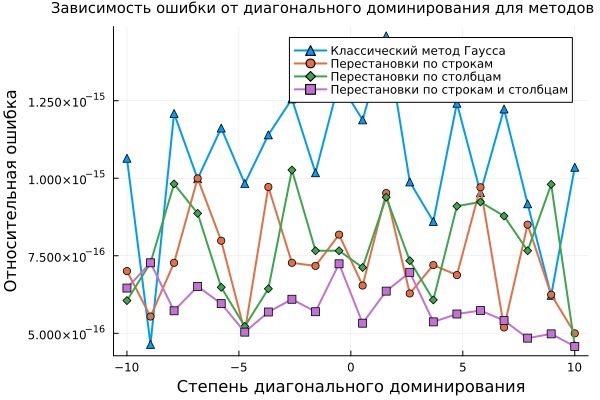
\includegraphics[width=0.8\textwidth]{img1}
\caption{Зависимость ошибки от диалонального доминирования для методов}
\label{fig:img1}
\end{figure}

\section{Выводы}\label{Sect::conclusion}

Проанализировав графики зависимостей ошибок разных методов от диагонального доминирования матриц можно сделать вывод о том, что самым оптимальным является модификация метода Гаусса перестановкой по строкам и столбцам, модификации метода Гаусса перестановкой по строкам или по столбцам относительно имеет близкую погрешность и классический метод Гаусса среди прочих имеет наибольшую относительную ошибку.

\end{document}
